%% Introdução: Uma Jornada Intelectual

\chapter*{Introdução: Uma Jornada Intelectual}
\addcontentsline{toc}{chapter}{Introdução: Uma Jornada Intelectual}

\epigrafe{Words are useless, especially sentences\\
They don't stand for anything\\
How can I explain how I feel?}{Madonna \& Björk, ``Bedtime Story''}

\epigrafe{As coisas só existem quando nomeadas.}{Graciliano Ramos, \textit{Vidas Secas}}

Este tratado nasce de uma longa jornada intelectual, das contradições e sínteses que marcaram meu percurso como estudioso da mente humana. Aos 17 anos, meu primeiro encontro com Bertrand Russell abriu-me as portas para a lógica, a filosofia da mente e da linguagem. Foi Russell quem me apresentou a Wittgenstein, cujo rigor lógico e insights sobre os limites da linguagem moldaram profundamente minha compreensão da relação entre pensamento e expressão.

As influências que fundamentam este trabalho são diversas e aparentemente paradoxais. Por um lado, a música expressando a frustração com a insuficiência da linguagem para capturar emoções profundas; por outro, a voz de Stephen Hawking no álbum ``The Division Bell'' do Pink Floyd, lembrando-nos em ``Keep Talking'' que a comunicação é o que nos torna humanos. Entre esses pólos, encontrei em Graciliano Ramos a compreensão de que as coisas só existem quando nomeadas, enquanto Guimarães Rosa me mostrava que a linguagem pode transcender suas próprias limitações através da inovação e poesia.

\section*{Influências Filosóficas}

Spinoza, talvez o grande injustiçado da filosofia, ofereceu-me uma visão integradora da mente e do corpo, dos afetos e da razão. Sua \textit{Ética}, com seu rigor geométrico aplicado a questões humanas, inspirou-me a buscar uma abordagem sistemática para fenômenos que muitos consideram demasiado subjetivos para análise formal. Já Habermas, cuja teoria da ação comunicativa só vim a compreender verdadeiramente anos após meus estudos de Administração Pública, forneceu-me o quadro conceitual para entender a linguagem como ação social transformadora.

\begin{center}
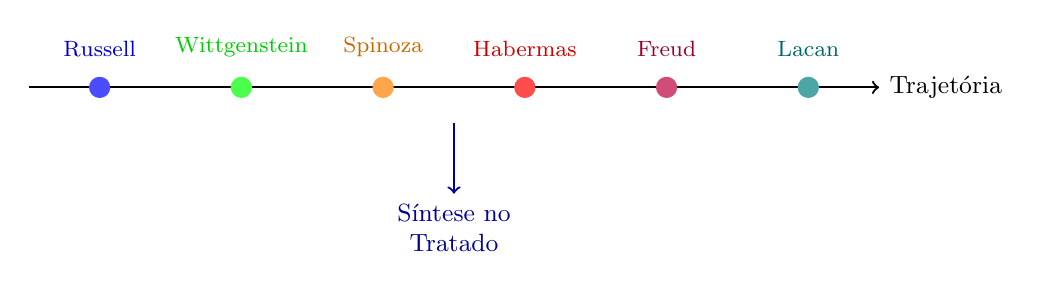
\begin{tikzpicture}[scale=0.9]
    % Linha do tempo das influências
    \draw[thick, ->] (0,0) -- (12,0) node[right] {\small Trajetória};

    % Pontos na linha
    \foreach \x/\nome/\cor in {1/Russell/blue, 3/Wittgenstein/green, 5/Spinoza/orange, 7/Habermas/red, 9/Freud/purple, 11/Lacan/teal} {
        \fill[\cor!70] (\x,0) circle (0.15);
        \node[\cor!80!black, above, font=\footnotesize] at (\x,0.3) {\nome};
    }

    % Seta para cima representando síntese
    \draw[thick, ->, blue!60!black] (6,-0.5) -- (6,-1.5) node[below, text width=3cm, align=center, font=\small] {Síntese no\\Tratado};
\end{tikzpicture}
\end{center}

\section*{Trajetória Acadêmica}

Meu percurso acadêmico reflete essa diversidade de interesses. A formação em Administração Pública na UNESP de Araraquara dotou-me de uma compreensão das estruturas sociais e institucionais que moldam nosso pensamento. Posteriormente, a Medicina na Estadual de Marília (FAMEMA) permitiu-me observar diretamente a interação entre corpo, mente e linguagem, especialmente nas manifestações psiquiátricas. Durante esse período, tive a oportunidade de estagiar na embaixada da ONU no UNFPA (Fundo de População das Nações Unidas), experiência que expandiu minha visão para dimensões globais das questões humanas. As posições como diretor nacional de estudantes, tanto de Administração Pública quanto de Medicina, proporcionaram-me uma perspectiva privilegiada sobre os desafios educacionais e profissionais desses campos.

\section*{O Paradoxo Produtivo}

Este tratado representa uma tentativa de sintetizar essas diversas influências em um quadro coerente. Busca-se aqui não apenas compreender a relação entre linguagem, cognição e emoção, mas propor uma nova forma de conceptualizar essa interdependência --- uma forma que reconhece tanto os limites quanto as potencialidades da linguagem na construção da subjetividade humana.

A tensão entre a insuficiência da linguagem e seu poder constitutivo não é um problema a ser resolvido, mas um paradoxo produtivo a ser explorado. É na navegação entre esses pólos que encontramos as possibilidades mais ricas para a compreensão e transformação da mente humana.

\begin{center}
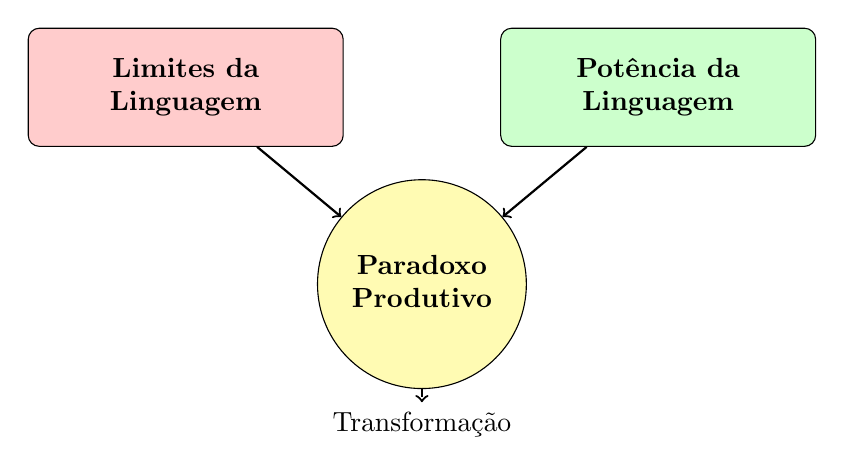
\begin{tikzpicture}[scale=1]
    % O paradoxo da linguagem
    \node[draw, rounded corners, fill=red!20, minimum width=4cm, minimum height=1.5cm] (lim) at (-3,0)
        {\begin{tabular}{c}\textbf{Limites da}\\\textbf{Linguagem}\end{tabular}};
    \node[draw, rounded corners, fill=green!20, minimum width=4cm, minimum height=1.5cm] (pot) at (3,0)
        {\begin{tabular}{c}\textbf{Potência da}\\\textbf{Linguagem}\end{tabular}};
    \node[draw, circle, fill=yellow!30, minimum size=2cm] (par) at (0,-2.5)
        {\begin{tabular}{c}\textbf{Paradoxo}\\\textbf{Produtivo}\end{tabular}};

    \draw[thick, ->] (lim) -- (par);
    \draw[thick, ->] (pot) -- (par);
    \draw[thick, ->, dashed] (par) -- (0,-4) node[below] {Transformação};
\end{tikzpicture}
\end{center}

Nas páginas que seguem, convido o leitor a embarcar nessa exploração, a questionar premissas estabelecidas e a considerar novas formas de entender a intrincada dança entre as palavras que usamos, os pensamentos que formulamos e as emoções que sentimos. Como Russell nos ensinou, a tarefa da filosofia não é fornecer respostas definitivas, mas clarificar questões fundamentais --- e é com esse espírito que ofereço este trabalho.

\vspace{2em}

\begin{flushright}
\textit{Gustavo Mendes e Silva, M.D.}
\end{flushright}

\nextpage
